\documentclass[utf8x]{beamer}

\mode<presentation>
{
  \usetheme{Warsaw}

  %\setbeamercovered{transparent}
}


\usepackage[english]{babel}

\usepackage[utf8x]{inputenc}

\usepackage{times}
\usepackage[T1]{fontenc}
\usepackage{ifthen}
\usepackage{fancyvrb}
\usepackage{color}
\usepackage{ulem}
\usepackage{listings}
\usepackage{amssymb}
\usepackage{booktabs}
\usepackage{wrapfig}
\usepackage{url}
\usepackage{alltt}
\usepackage{tikz}
\usetikzlibrary{arrows,positioning,shadows,shapes,calc,backgrounds,fit}

%\input{pygmentheader.tex}

\title[PyPy Implements Dynamic Languages Using a Tracing JIT]{
PyPy's Approach to \\
Implementing Dynamic Languages \\
Using a Tracing JIT Compiler}

\author{Carl Friedrich Bolz}

\institute[Heinrich-Heine-Universität Düsseldorf]
{
  Institut für Informatik\\
  Heinrich-Heine-Universität Düsseldorf
}

\date{
%\includegraphics[scale=0.25]{figures/hpi_logo_kl.jpg}\\
%IBM Watson Research Center, February 9th, 2011
Microsoft Research, January 31st, 2011
}

%\pgfdeclareimage[height=0.5cm]{pypy-logo}{image/py-web.png}
%\logo{\pgfuseimage{pypy-logo}}



% Delete this, if you do not want the table of contents to pop up at
% the beginning of each subsection:
%\AtBeginSubsection[]
%{
%  \begin{frame}<beamer>
%    \frametitle{Outline}
%    \tableofcontents[currentsection,currentsubsection]
%  \end{frame}
%}


% If you wish to uncover everything in a step-wise fashion, uncomment
% the following command: 

%\beamerdefaultoverlayspecification{<+->}


\begin{document}

\begin{frame}
  \titlepage
\end{frame}


\begin{frame}
  \frametitle{Scope}
  This talk is about:

  \begin{itemize}
  \item implementing dynamic languages \par(with a focus on complicated ones)
  \item in a context of limited resources \par(academic, open source, or
    domain-specific)
  \item imperative, object-oriented languages
  \item single-threaded implementations
  \end{itemize}
  \pause
  \begin{block}{Goals}
    Reconciling:
    \begin{itemize}
    \item flexibility, maintainability (because languages evolve)
    \item simplicity (because teams are small)
    \item performance
    \end{itemize}
  \end{block}
\end{frame}

\begin{frame}
  \frametitle{Outline}
  \tableofcontents[pausesections]
  % You might wish to add the option [pausesections]
\end{frame}

\section{The Difficulties of Implementing Dynamic Languages}

\subsection{Technical Factors}

\begin{frame}
  \frametitle{What is Needed Anyway}
  A lot of things are not really different from other languages:
  \begin{itemize}
      \item lexer, parser
      \item (bytecode) compiler
      \item garbage collector
      \item object system
  \end{itemize}
\end{frame}

% say, but don't write:
% from pypy perspective, but trying to do a general analysis
% feedback/discussion welcome
%  XXX random thought: a lot of semantics implemented on VM level, operations
%  XXX other direction: PyPy has granularity issues in opposite direction


\begin{frame}
  \frametitle{Control Flow}
    \begin{itemize}
        \item every language implementation needs a way to implement the control flow of the language
        \item trivially and slowly done in interpreters with AST or bytecode
        \item technically very well understood
        \item sometimes small difficulties, like generators in Python
        \pause
        \item some languages have more complex demands\\
        but this is rare
        \item examples: Prolog
    \end{itemize}
\end{frame}

\begin{frame}
  \frametitle{Late Binding}
  \begin{itemize}
      \item lookups can be done only at runtime
      \item historically, dynamic languages have moved to ever later binding times
      \item a large variety of mechanisms exist in various languages
      \item mechanism are often very ad-hoc because \\
      "it was easy to do in an interpreter"
  \end{itemize}
\end{frame}

\begin{frame}
  \frametitle{Late Binding in Python}
  In Python, the following things are late bound
  \begin{itemize}
      \item global names
      \item modules
      \item instance variables
      \item methods
      \pause
      \item the class of objects
      \item class hierarchy
  \end{itemize}
\end{frame}


\begin{frame}
  \frametitle{Dispatching}
  \begin{itemize}
      \item dispatching is a very important special case of late binding
      \item how are the operations on objects implemented?
      \item this is usually very complex, and different between languages
      \pause
      \item operations are internally split up into one or several lookup and call steps
      \item a huge space of paths ensues
      \item most of the paths are uncommon
  \end{itemize}
\end{frame}

\begin{frame}
  \frametitle{Example: Attribute Reads in Python}
  What happens when an attribute \texttt{x.m} is read? (simplified)
  \begin{itemize}
      \item check for the presence of \texttt{x.\_\_getattribute\_\_}, if there, call it
      \pause
      \item look for the name of the attribute in the object's dictionary, if it's there, return it
      \pause
      \item walk up the MRO of the object and look in each class' dictionary for the attribute
      \pause
      \item if the attribute is found, call its \texttt{\_\_get\_\_} attribute and return the result
      \pause
      \item if the attribute is not found, look for \texttt{x.\_\_getattr\_\_}, if there, call it
      \pause
      \item raise an \texttt{AttributeError}
  \end{itemize}
\end{frame}

\begin{frame}
  \frametitle{Example: Addition in Python}
  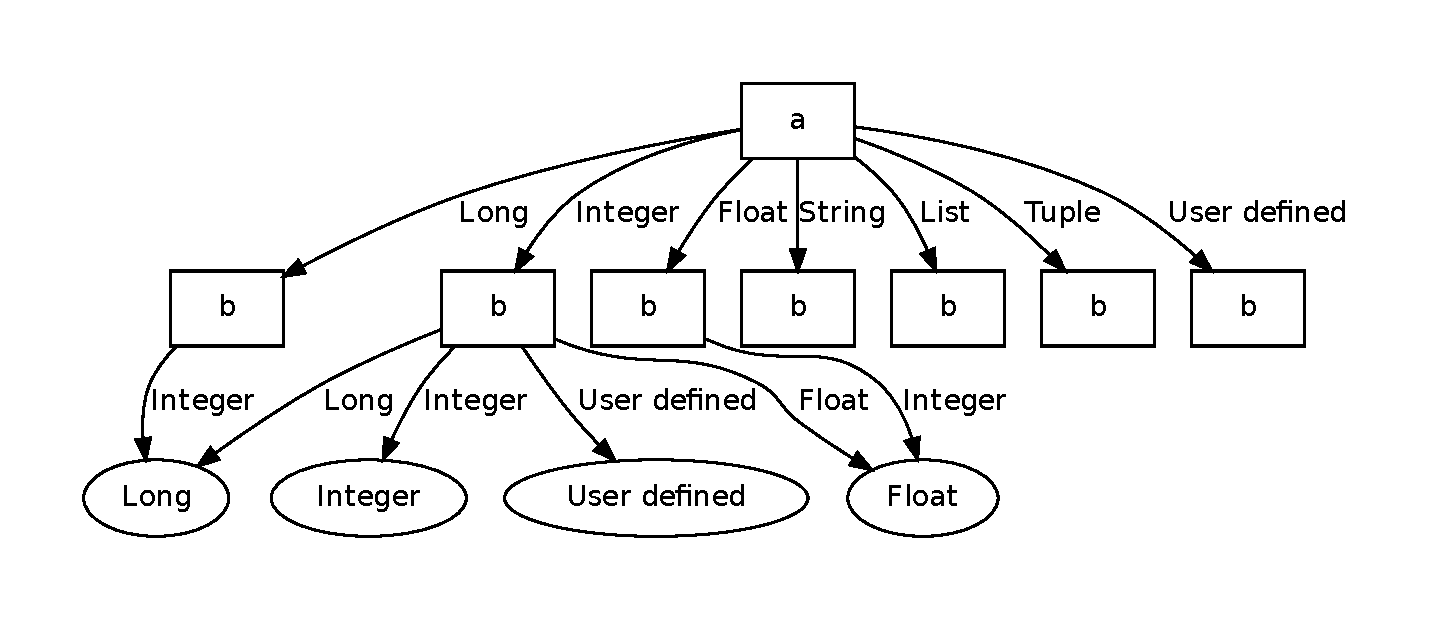
\includegraphics[scale=0.5]{figures/add.pdf}
\end{frame}

\begin{frame}
  \frametitle{Dependencies Between Subsequent Dispatches}
  \begin{itemize}
      \item one dispatch operation is complex
      \item many in a sequence are worse
      \item take \texttt{(a + b) + c}
      \item the dispatch decision of the first operation influences the second
  \end{itemize}
\end{frame}




\begin{frame}
  \frametitle{Boxing of Primitive Values}
  \begin{itemize}
      \item primitive values often need to be boxed,\\
      to ensure uniform access
      \item a lot of pressure is put on the GC by arithmetic
      \item need a good GC (clear anyway)
      \item in arithmetic, lifetime of boxes is known
  \end{itemize}
%  \pause
%  \begin{block}{Escape Analysis?}
%    \begin{itemize}
%        \item should help in theory
%        \item nearly always there are some unlikely paths,\\
%        that lead to escapes
%        \item this is often due to user-overriding of operations
%    \end{itemize}
%  \end{block}
\end{frame}

\begin{frame}
  \frametitle{Escaping Paths}
  \begin{itemize}
      \item considering again \texttt{(a + b) + c}
      \item assume \texttt{a} and \texttt{b} are ints
      \item then the result should not be allocated
      \item escaping path: if \texttt{c} has a user-defined class
  \end{itemize}
\end{frame}



\begin{frame}
  \frametitle{(Frames)}
  \begin{itemize}
      \item side problem:
      \item many languages have reified frame access
      \item e.g. Python, Smalltalk, Ruby, ...
      \item support for in-language debuggers
      \item in an interpreter these are trivial,\\
      because the interpreter needs them anyway
      \item how should reified frames work efficiently when a compiler is used?
  \end{itemize}
\end{frame}

%\begin{frame}
%  \frametitle{(Fast Access to Native Libraries)}
%  \begin{itemize}
%      \item another side problem
%      \item how can native libraries be accessed efficiently?
%      \item important in dynamic languages, because they are often used as glue
%      \item even more important in browser, to interact with the DOM
%      \item can be solved either by compiling extensions, or via an FFI
%      \item both not very efficient
%  \end{itemize}
%\end{frame}

\subsection{Requirements}

\begin{frame}
  \frametitle{Summarizing the Requirements}
  \begin{enumerate}
      \item control flow
      \item late binding
      \item \textbf{dispatching}
      \item \textbf{dependencies between subsequent dispatches}
      \item boxing
      \item (reified frames)
%      \item (access to native libraries)
  \end{enumerate}
\end{frame}


\section{Approaches For Dynamic Language Implementation}

\begin{frame}
  \frametitle{Common Approaches to Language Implementation}
  \begin{itemize}
    \item Using C/C++
    \begin{itemize}
      \item for an interpreter
      \item for a static compiler
      \item for a method-based JIT
      \item for a tracing JIT
    \end{itemize}
    \item Building on top of a general-purpose OO VM
  \end{itemize}
\end{frame}

\begin{frame}
  \frametitle{Common Approaches to Language Implementation}
  \begin{block}{
    Using C/C++}
    \begin{itemize}
    \item CPython (interpreter)
    \item Ruby (interpreter)
    \item V8 (method-based JIT)
    \item TraceMonkey (tracing JIT)
    \item ...
    %\item but also: Scheme48, Squeak (interpreters)
    \end{itemize}
  \end{block}
  \pause
  \begin{block}{Building on top of a general-purpose OO VM}
    \begin{itemize}
    \item Jython, IronPython
    \item JRuby, IronRuby
    \item various Prolog, Lisp, even Smalltalk implementations
    \end{itemize}
  \end{block}
\end{frame}

\subsection{Implementing VMs in C/C++}

\begin{frame}
  \frametitle{Implementing VMs in C}
  When writing a VM in C it is hard to reconcile our goals
  \begin{itemize}
  \item flexibility, maintainability
  \item simplicity
  \item performance
  \end{itemize}
  \pause
  \begin{block}{Python Case}
    \begin{itemize}
    \item \alert{CPython} is a very simple bytecode VM, performance not great
    \item \alert{Psyco} is a just-in-time-specializer, very complex, hard to
      maintain, but good performance
    \item \alert{Stackless} is a fork of CPython adding microthreads. It was
    never incorporated into CPython for complexity reasons
    \end{itemize}
  \end{block}
\end{frame}

\begin{frame}
  \frametitle{Interpreters in C/C++}
  \begin{itemize}
      \item mostly very easy
      \item well understood problem
      \item portable, maintainable
      \item slow
  \end{itemize}

\end{frame}


%\begin{frame}
%  \frametitle{Fixing of Early Design Decisions}
%  \begin{itemize}
%  \item when starting a VM in C, many design decisions need to be made upfront
%  \item examples: memory management technique, threading model
%  \item such decisions are manifested throughout the VM source
%  \item very hard to change later
%  \item low level details mixed with language semantics
%  \end{itemize}
%  \pause
%  \begin{block}{Python Case}
%    \begin{itemize}
%    \item CPython uses reference counting, increfs and decrefs everywhere
%    \item CPython uses OS threads with one global lock, hard to change to
%      lightweight threads or finer locking
%    \end{itemize}
%  \end{block}
%\end{frame}


\begin{frame}
  \frametitle{How do Interpreters Meet the Requirements?}
  \begin{enumerate}
      \item \alert{control flow slowed by bytecode or AST dispatch overhead}
      \item \alert{late binding works but slow}
      \item \alert{dispatching works but slow}
      \item \alert{no special dependencies support}
      \item \alert{everything is boxed}
      \item \alert{reified frames are easy but slow}
%      \item \alert{access to native libraries easy but slow}
  \end{enumerate}
\end{frame}



\begin{frame}
  \frametitle{Static Compilers to C/C++}
  \begin{itemize}
      \item first reflex of many people is to blame it all on bytecode dispatch overhead
      \item thus static compilers are implemented that reuse the object model of an interpreter
      \item gets rid of interpretation overhead only
      \item seems to give about 2x speedup
      \pause
      \item dispatch, late-binding and boxing only marginally improved
      \item static analysis mostly never works
%      \item often easy access to native libraries
  \end{itemize}
  \pause
  \begin{block}{Python Case}
    \begin{itemize}
    \item \alert{Cython}, \alert{Pyrex} are compilers\\
    from large subsets of Python to C
    \item lots of older experiments, most discontinued
    \end{itemize}
  \end{block}
\end{frame}


\begin{frame}
  \frametitle{How do Static Compilers Meet the Requirements?}
  \begin{enumerate}
      \item control flow works well
      \item \alert{late binding not improved}
      \item \alert{dispatching not improved}
      \item \alert{dependencies not improved}
      \item \alert{everything is boxed}
      \item \alert{reified frames often not supported}
%      \item direct access to native libraries
  \end{enumerate}
\end{frame}


\subsection{Method-Based JIT Compilers}

\begin{frame}
  \frametitle{Method-Based JIT Compilers}
  \begin{itemize}
      \item to fundamentally attack some of the problems, \\
      a dynamic compiler is needed
      \item a whole new can of worms
      \pause
      \begin{itemize}
          \item type profiling
          \item inlining based on that
          \item general optimizations
          \item complex backends
      \end{itemize}
      \item very hard to pull off for a volunteer team
  \end{itemize}
  \pause
  \begin{block}{Examples}
      \begin{itemize}
          \item Smalltalk and SELF JITs
          \item V8 and JägerMonkey
          \item Psyco, sort of
      \end{itemize}
  \end{block}
\end{frame}

\begin{frame}
  \frametitle{Compilers are a bad encoding of Semantics}
  \begin{itemize}
  \item to improve all complex corner cases of the language, \\
  a huge effort is needed
  \item often needs a big "bag of tricks"
  \item the interactions between all tricks is hard to foresee
  \item the encoding of language semantics in the compiler is thus often obscure and hard to change
  \end{itemize}
  \pause
  \begin{block}{
    Python Case}
    \begin{itemize}
    \item Psyco is a dynamic compiler for Python
    \item synchronizing with CPython's development is a lot of effort
    \item many of CPython's new features not supported well
    \item not ported to 64-bit machines, and probably never will
    \end{itemize}
  \end{block}
\end{frame}

\begin{frame}[containsverbatim]
  \frametitle{Method-Based JITs and Dispatching Dependencies}
\begin{verbatim}
    x = add(a, b)
    r = add(x, c)
\end{verbatim}
\end{frame}

\begin{frame}[containsverbatim, plain]
  \frametitle{Method-Based JITs and Dispatching Dependencies}
\begin{verbatim}
    if isinstance(a, Integer):
        if isinstance(b, Integer):
            x = Integer(<perform int addition>)
        else:
            x = Float(<perform float addition>)
    else:
        x = Float(<perform float addition>)
    # x can be Float or Integer here
    if isinstance(x, Integer):
        if isinstance(c, Integer):
            r = Integer(<perform int addition>)
        else:
            r = Float(<perform float addition>)
    else:
        r = Float(<perform float addition>)
\end{verbatim}
\end{frame}

\begin{frame}
  \frametitle{How do Method-Based JIT Compilers Meet the Requirements?}
  \begin{enumerate}
      \item control flow works well
      \item late binding can be handled
      \item dispatching can be handled
      \item \alert{dependencies not necessarily improved}
      \item boxing hard to support
      \item \alert{reified frames hard to support}
%      \item \alert{access to native libraries not improved}
  \end{enumerate}
\end{frame}



\subsection{Tracing JIT Compilers}

\begin{frame}
  \frametitle{Tracing JIT Compilers}
  \begin{itemize}
      \item relatively recent approach to JIT compilers
      \item pioneered by Michael Franz and Andreas Gal for Java
      \item turned out to be well-suited for dynamic languages
  \end{itemize}
  \pause
  \begin{block}{Examples}
      \begin{itemize}
          \item \alert{TraceMonkey}
          \item \alert{LuaJIT}
          \item \alert{SPUR}, sort of
          \item \alert{PyPy}, sort of
      \end{itemize}
  \end{block}
\end{frame}

\begin{frame}
    \frametitle{Tracing JIT Compilers}
    \begin{itemize}
    \item idea from Dynamo project: \\
    dynamic rewriting of machine code
    \item conceptually simpler than type profiling
    \end{itemize}
    \pause
    \begin{block}{Basic Assumption of a Tracing JIT}
        \begin{itemize}
        \item programs spend most of their time executing loops
        \item several iterations of a loop are likely to take similar code paths
        \end{itemize}
    \end{block}
\end{frame}

\begin{frame}
    \frametitle{Tracing VMs}
    \begin{itemize}
    \item mixed-mode execution environment
    \item at first, everything is interpreted
    \item lightweight profiling to discover hot loops
    \item code generation only for common paths of hot loops
    \item when a hot loop is discovered, start to produce a trace
    \end{itemize}
\end{frame}

\begin{frame}
    \frametitle{Tracing}
    \begin{itemize}
    \item a \emph{trace} is a sequential list of operations
    \item a trace is produced by recording every operation the interpreter executes
    \item tracing ends when the tracer sees a position in the program it has seen before
    \item a trace thus corresponds to exactly one loop
    \item that means it ends with a jump to its beginning
    \end{itemize}
    \pause
    \begin{block}{Guards}
        \begin{itemize}
        \item the trace is only one of the possible code paths through the loop
        \item at places where the path \emph{could} diverge, a guard is placed
        \end{itemize}
    \end{block}
\end{frame}

\begin{frame}
    \frametitle{Code Generation and Execution}
    \begin{itemize}
    \item being linear, the trace can easily be turned into machine code
    \item execution stops when a guard fails
    \item after a guard failure, go back to interpreting program
    \end{itemize}
\end{frame}

\begin{frame}
  \frametitle{Dealing With Control Flow}
  \begin{itemize}
      \item an if statement in a loop is turned into a guard
      \item if that guard fails often, things are inefficient
      \item solution: attach a new trace to a guard, if it fails often enough
      \item new trace can lead back to same loop
      \item or to some other loop
  \end{itemize}
\end{frame}

%\begin{frame}
%  \frametitle{Stages of Execution}
%  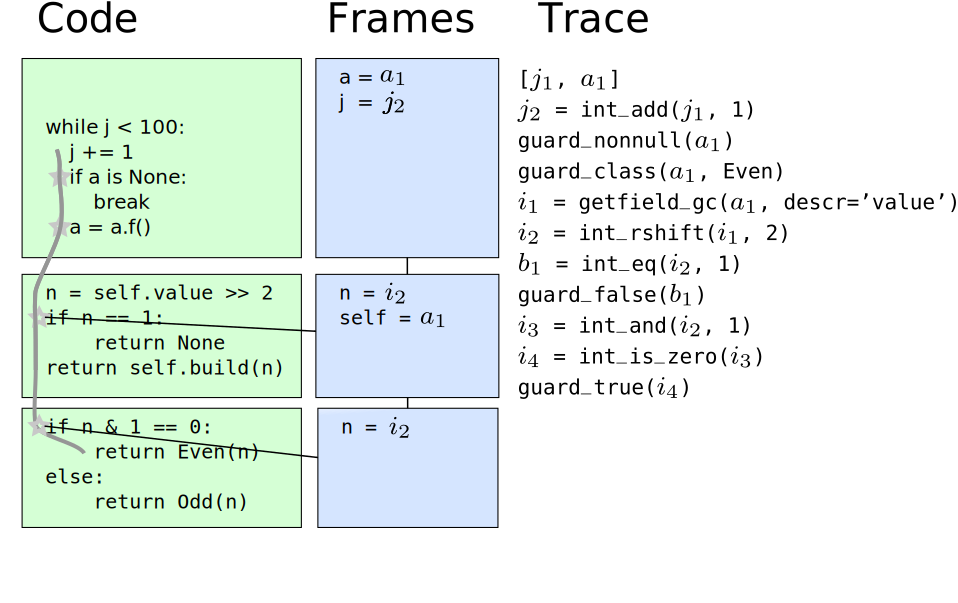
\includegraphics[scale=0.5]{figures/tracing.pdf}
%\end{frame}

\begin{frame}
  \frametitle{Dispatching in a Tracing JIT}
  \begin{itemize}
      \item trace contains bytecode operations
      \item bytecodes often have complex semantics
      \item optimizer often type-specializes the bytecodes
      \item according to the concrete types seen during tracing
      \item need to duplicate language semantics in optimizer for that
  \end{itemize}
\end{frame}


\begin{frame}
  \frametitle{Dispatching Dependencies in a Tracing JIT}
  \begin{itemize}
      \item one consequence of the tracing approach:
      \item paths are split aggressively
      \item control flow merging happens at beginning of loop only
      \item after a type check, the rest of the trace can assume that type
      \item only deal with paths that are actually seen
  \end{itemize}
\end{frame}

\begin{frame}
  \frametitle{Boxing Optimizations in a Tracing JIT}
  \begin{itemize}
      \item possibility to do escape analysis within the trace
      \item only optimize common path
      \item i.e. the one where the object doesn't escape
  \end{itemize}
\end{frame}


\begin{frame}
    \frametitle{Advantages of Tracing JITs}
    \begin{itemize}
    \item can be added to an existing interpreter unobtrusively
    \item interpreter does most of the work
    \item automatic inlining
    \item deals well with finding the few common paths through the large space
    \end{itemize}
\end{frame}

\begin{frame}
    \frametitle{Bad Points of the Approach}
    \begin{itemize}
        \item switching between interpretation and machine code execution takes time
        \item problems with really complex control flow
        \item granularity issues: often interpreter bytecode is too coarse
        \item if this is the case, the optimizer needs to carefully re-add the decision tree
    \end{itemize}
\end{frame}

\begin{frame}
  \frametitle{How do Tracing JITs Meet the Requirements?}
  \begin{enumerate}
      \item control flow works rather well
      \item late binding can be handled
      \item dispatching can be handled
      \item dependencies improved by path splitting
      \item unboxing optimization much simpler
      \item reified frames can be implemented \\
      by falling back to the interpreter
%      \item \alert{access to native libraries not improved}
  \end{enumerate}
\end{frame}


\subsection{Building on Top of an OO VM}

\begin{frame}
  \frametitle{Implementing Languages on Top of OO VMs}
  \begin{itemize}
  \item approach: implement on top of the JVM or the CLR
  \item usually by compiling to the target bytecode
  \item plus an object model implementation
  \item brings its own set of benefits of problems
  \end{itemize}
  \pause
  \begin{block}{
    Python Case}
    \begin{itemize}
    \item \alert{Jython} is a Python-to-Java-bytecode compiler
    \item \alert{IronPython} is a Python-to-CLR-bytecode compiler
    \end{itemize}
  \end{block}
\end{frame}

\begin{frame}
  \frametitle{Benefits of Implementing on Top of OO VMs}
  \begin{itemize}
  \item higher level of implementation
  \item the VM supplies a GC and a JIT
  \item better interoperability than what the C level provides
  \end{itemize}
  \pause
  \begin{block}{
    Python Case}
    \begin{itemize}
    \item both Jython and IronPython integrate well with their host OO VM
    \item both have proper threading
    \end{itemize}
  \end{block}
\end{frame}

\begin{frame}
  \frametitle{The Problems of OO VMs}
  \begin{itemize}
      \item often hard to map concepts of the dynamic language
      \item performance not improved because of the semantic mismatch
      \item untypical code in most object models
      \item object model typically has many megamorphic call sites
      \pause
      \item escape analysis cannot help with boxing,\\
      due to escaping paths
      \item to improve, very careful manual tuning is needed
      \item VM does not provide enough customization/feedback
  \end{itemize}
\end{frame}

\begin{frame}
  \frametitle{Examples of Problems}
  \begin{itemize}
      \item both Jython and IronPython are quite a bit slower than CPython
      \item IronPython misses reified frames
      \pause
      \item for languages like Prolog it is even harder to map the concepts
  \end{itemize}
\end{frame}

 
\begin{frame}
  \frametitle{The Future of OO VMs?}
  \begin{itemize}
  \item the problems described might improve in the future
  \item JVM will add extra support for more languages
  \item i.e. tail calls, \texttt{InvokeDynamic}, ...
  \item has not really landed yet
  \item good performance needs a huge amount of tweaking
  \item controlling the VM's behaviour is brittle:\\
  VMs not meant for people who care about exact shape of assembler
  \end{itemize}
  \pause
  \begin{block}{Ruby Case}
    \begin{itemize}
    \item JRuby tries really hard to be a very good implementations
    \item took an enormous amount of effort
    \item tweaking is essentially Hotspot-specific
    \end{itemize}
  \end{block}
\end{frame}

\begin{frame}
  \frametitle{How do OO VMs Meet the Requirements?}
  \begin{enumerate}
      \item control flow works well
      \item late binding can be handled with a lot of effort
      \item dispatching can be handled with a lot of effort
      \item \alert{dependencies not improved}
      \item \alert{boxing not necessarily improved}
      \item \alert{reified frames are inefficient}
%      \item access to native libraries not improved, but VM libraries help
  \end{enumerate}
\end{frame}

\section{PyPy's Approach to VM Construction}


\begin{frame}
  \frametitle{The PyPy Project}
  \begin{itemize}
      \item started in 2003, received funding from the EU, Google, Nokia and some smaller companies
      \item goal: "The PyPy project aims at producing a flexible and fast Python implementation."
      \item technology should be reusable for other dynamic languages
  \end{itemize}
  \pause
  \begin{block}{Language Status}
    \begin{itemize}
        \item the fastest Python implementation, very complete
        \item contains a reasonably good Prolog
        \item full Squeak, but no JIT for that yet
        \item various smaller experiments (JavaScript, Scheme, Haskell)
    \end{itemize}
      
  \end{block}
\end{frame}

\begin{frame}
  \frametitle{PyPy's Approach to VM Construction}
  \emph{Goal: achieve flexibility, simplicity and performance together}

  \begin{itemize}
  \item Approach: auto-generate VMs from high-level descriptions of the language
  \item ... using meta-programming techniques and \emph{aspects}
  \item high-level description: an interpreter written in a high-level language
  \item ... which we translate (i.e.\ compile) to a VM running in various target
    environments, like C/Posix\pause, CLR, JVM
  \end{itemize}
\end{frame}

\begin{frame}
  \frametitle{PyPy}
  \begin{itemize}
  \item PyPy = Python interpreter written in RPython + translation toolchain
    for RPython
  \end{itemize}
  \pause
  \begin{block}{What is RPython}
    \begin{itemize}
    \item RPython is a (large) subset of Python
    \item subset chosen in such a way that type-inference can be performed
    \item still a high-level language (unlike SLang or PreScheme)
    \end{itemize}
  \end{block}
\end{frame}

\begin{frame}
  \frametitle{Auto-generating VMs}
  \begin{itemize}
  \item we need a custom \emph{translation toolchain} to compile the interpreter
    to a full VM
  \item many aspects of the final VM are orthogonal from the interpreter source:
    they are inserted during translation
  \end{itemize}
  \pause
  \begin{block}{
    Examples}
    \begin{itemize}
    \item Garbage Collection strategy
%    \item Threading models (e.g.\ coroutines with CPS...)
    \item non-trivial translation aspect: auto-generating a tracing JIT compiler from
      the interpreter
    \end{itemize}
  \end{block}
\end{frame}


\begin{frame}
  \frametitle{Good Points of the Approach}
  {\bf Simplicity:} separation of language semantics from low-level details
  \pause

  {\bf Flexibility} high-level implementation language eases things (meta-programming)
  \pause

  {\bf Performance:} ``reasonable'' baseline performance, can be very good with JIT
\end{frame}


\begin{frame}[plain]
  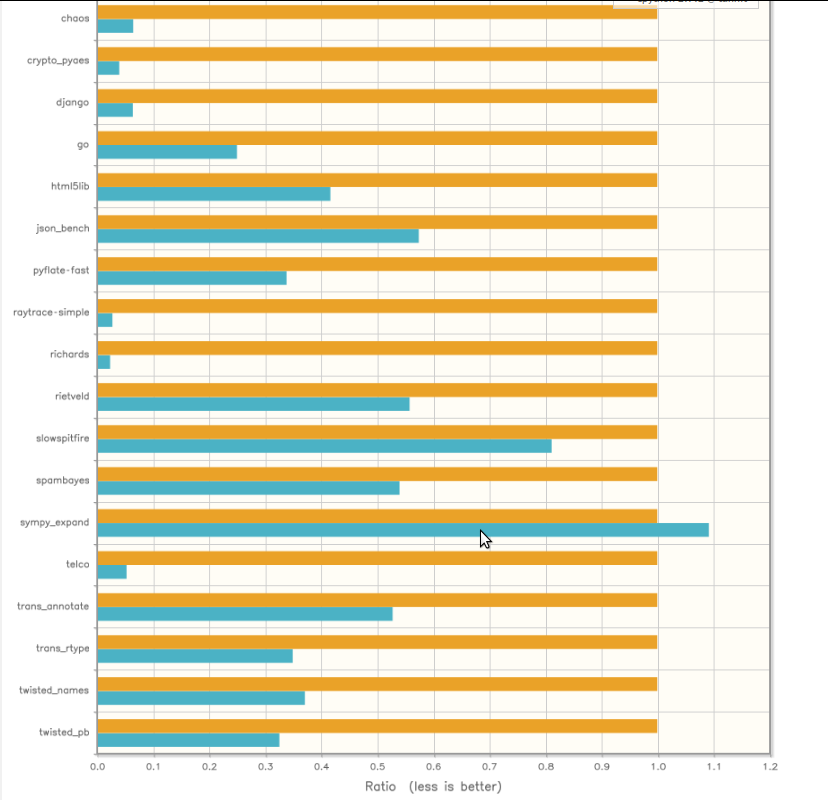
\includegraphics[scale=0.3]{figures/all_numbers.png}
\end{frame}

\subsection{PyPy's Meta-Tracing JIT Compiler}

%\begin{frame}
%  \frametitle{Example}
%XXX the idea of this section is to have a running example of a small
%interpreter that is extended with language constructs to provide examples for
%all the technologies
%
%\end{frame}

\begin{frame}
  \frametitle{Meta-Tracing}
  Problems of Tracing JITs:
  \begin{itemize}
      \item specific to one language's bytecode
      \item bytecode has wrong granularity
      \item internals of an operation not visible in trace
  \end{itemize}
  \pause
  \begin{block}{PyPy's Idea:}
      \begin{itemize}
          \item write interpreters in RPython
          \item trace the execution of the RPython code
          \item using one generic RPython tracer
          \item the process is customized via hints in the interpreter
          \item no language-specific bugs
      \end{itemize}
  \end{block}
\end{frame}

\begin{frame}
  \frametitle{Interpreter Overhead}
  \begin{itemize}
      \item most immediate problem with meta-tracing
      \item interpreter typically has a bytecode dispatch loop
      \item not a good idea to trace that
      \pause
      \item solved by a simple trick:
      \item \emph{unroll} the bytecode dispatch loop
      \item control flow then taken care of
  \end{itemize}
\end{frame}

\begin{frame}
  \frametitle{Optimizing Late Binding and Dispatching}
  \begin{itemize}
      \item late binding and dispatching code in the interpreter is traced
      \item as in a normal tracing JIT, the meta-tracer is good at picking common paths
      \item a number of hints to fine-tune the process
  \end{itemize}
\end{frame}

\begin{frame}
  \frametitle{Optimizing Boxing Overhead}
  \begin{itemize}
      \item boxing optimized by a powerful general optimization on traces
      \item tries to defer allocations for as long as possible
      \item allocations only happen in those (rare) paths where they are needed
  \end{itemize}
  \pause
  \begin{block}{Use Cases}
      \begin{itemize}
          \item arithmetic
          \item argument holder objects
          \item frames of inlined functions
      \end{itemize}
  \end{block}
\end{frame}

\begin{frame}
  \frametitle{Dealing With Reified Frames}
  \begin{itemize}
      \item interpreter needs a frame object to store its data anyway
      \item those frame objects are specially marked
      \item JIT special-cases them
      \item their attributes can live in CPU registers/stack
      \item on reflective access, machine code is left, interpreter continues
      \pause
      \item nothing deep, but a lot of engineering
  \end{itemize}
\end{frame}

\begin{frame}
  \frametitle{Feedback from the VM}
  \begin{itemize}
      \item in the beginning the hints are often not optimal yet
      \item to understand how to improve them, the traces must be read
      \item traces are in a machine-level intermediate representation
      \item not machine code
      \item corresponds quite closely to RPython interpreter code
      \item visualization and profiling tools
  \end{itemize}
\end{frame}


%\subsection{Customizing the Tracing of the Interpreter}
%
%\begin{frame}
%  \frametitle{Customizing the Tracing of the Interpreter}
%  - general building blocks for implementing many different dynamic languages well
%
%  - more expedient than minimal
%
%  without hints, behaviour is correct but not very fast
%\end{frame}
%
%
%\begin{frame}
%  \frametitle{The Extent of Tracing}
%  \begin{itemize}
%      \item tracer always starts at bytecode dispatch loop
%      \item at any interpreter-level function call, the tracer can decide to trace into call, or not
%      \item tracing should not continue arbitrarily deep into implementation of operations
%      \pause
%      \item basic mechanism: stop at functions that contain loops
%      \item hint to stop tracing explicitly
%      \item hint to force tracing into function with loops, unrolling them
%  \end{itemize}
%\end{frame}
%
%\begin{frame}
%  \frametitle{Example}
%  XXX
%\end{frame}
%
%
%\begin{frame}
%  \frametitle{Mechanisms for Dispatching and Late-Binding}
%  - tracing time computation
%
%  - promotion, turn a variable into a constant to insert a guard
%
%  - immutability, to fold away reads out of constants
%
%  - pure function hints, remove function calls if the arguments are pure
%
%\end{frame}
%
%\begin{frame}
%  \frametitle{Example Promotion}
%  XXX maps
%\end{frame}
%
%\begin{frame}
%  \frametitle{Example Immutability}
%  XXX code objects
%\end{frame}
%
%
%\begin{frame}
%  \frametitle{Example Pure Function}
%  XXX version tags
%\end{frame}
%
%\begin{frame}
%  \frametitle{Out-of-Line Guards}
%  - soon: slow-changing fields into out-of-line guards
%\end{frame}
%
%\begin{frame}
%  \frametitle{Example Out-of-Line Guards}
%  XXX version tags
%\end{frame}

\begin{frame}
  \frametitle{Drawbacks / Open Issues / Further Work}
  \begin{itemize}
  \item writing the translation toolchain in the first place takes lots of effort
    (but it can be reused)
  \item writing a good GC was still necessary, not perfect yet
  \item dynamic compiler generation seems to work now, but took \emph{very} long to get right
  \item granularity of tracing is sometimes not optimal, very low level
  \end{itemize}
\end{frame}

\begin{frame}
  \frametitle{Conclusion}
  \begin{itemize}
      \item PyPy solves many of the problems of dynamic language implementations
      \item it uses a high-level language
      \begin{itemize}
          \item to ease implementation
          \item for better analyzability
      \end{itemize}
      \item it gives good feedback to the language implementor
      \item and provides various mechanisms to express deeply different language semantics
      \pause
      \item only one solution in this design space (SPUR is another)
      \item more experiments needed
  \end{itemize}
\end{frame}


\end{document}


